%% ============================================================================
%% FULL PAPER — ASSEMBLED DRAFT (LaTeX, 2026-06-08) — Overleaf-ready.
%% Generated from paper_workspace/drafts/*.md. Compiles with pdfLaTeX (elsarticle).
%% Open items are rendered in red via \todo{...} so they are visible and the file
%% still compiles. Source of truth for prose: drafts/ ; for numbers: 00_design/G1.
%% Section cross-references use \ref{} (auto-numbered), so LaTeX numbering is correct
%% even though Data/Results/Discussion shift vs the markdown's provisional "5b" scheme.
%% ============================================================================
\documentclass[review,authoryear]{elsarticle}

\usepackage[utf8]{inputenc}
\usepackage[T1]{fontenc}
\usepackage{amsmath,amssymb}
\usepackage{booktabs}
\usepackage{graphicx}
\usepackage{float}
\usepackage{hyperref}
\usepackage{multirow}
\usepackage{siunitx}
\usepackage{xcolor}
\usepackage{gensymb}
\usepackage{comment}
\usepackage[margin=1in]{geometry}

% Visible placeholder for anything still pending (G5 lit, tables, figures, abstract).
\newcommand{\todo}[1]{{\color{red}\textbf{[#1]}}}
\newcommand{\fcr}{\mathrm{FCR}}

\journal{Transportation Research Part C: Emerging Technologies}

% Suppress the elsarticle "Preprint submitted to ... <date>" footer.
\makeatletter
\def\ps@pprintTitle{%
  \let\@oddhead\@empty
  \let\@evenhead\@empty
  \def\@oddfoot{}%
  \let\@evenfoot\@oddfoot}
\makeatother

\begin{document}

\begin{frontmatter}

\title{Maritime Speed Optimization Under Sea Conditions Uncertainty}

\author[tau]{Ami Shafir}
\author[tau]{Tal Raviv}
\address[tau]{Faculty of Engineering, Tel Raviv University, Tel Aviv, Israel}

\begin{abstract}
Ship speed is the most immediate lever for cutting marine fuel use and greenhouse-gas emissions, but
the convexity of fuel consumption in speed --- which makes a constant speed optimal in uniform
conditions --- penalises a constant speed when weather varies along a voyage. This suggests that
resolving the speed decision finely, cell by cell, should save fuel; yet state-of-the-art methods hold
speed constant across coarse forecast-cycle stages, because the space of candidate speed profiles grows
exponentially with the number of stages, and whether finer resolution actually pays has not been
established. We formulate deterministic speed control as a shortest-path problem on a directed acyclic
graph in the time--distance plane, allowing the speed to change at every weather-cell crossing and
heading change while remaining solvable in a single polynomial-time Bellman sweep. We embed this
program (SR: speed chosen freely at every boundary) in a rolling-horizon scheme driven by real
operational weather forecasts, and evaluate it with a data-driven voyage simulation against both a
fixed-speed operational policy and the state-of-the-art per-block formulation of \citet{luo2024} (Luo:
speed held constant within each forecast-cycle block), over nineteen voyages on two contrasting routes.
Under perfect foresight SR burned less fuel than Luo on all nineteen voyages --- by up to a
few percent of voyage fuel, several tonnes of bunker fuel per voyage --- with the saving growing with
weather variability. The advantage persisted under realistic, imperfect-forecast operation, where SR
re-planning reduced fuel on 17 of 19 voyages while Luo, though it
re-planned more often, did not. The granularity of the speed decision, not the quality of the forecast
data, is the binding factor.
\end{abstract}

\begin{keyword}
ship speed optimization \sep dynamic programming \sep rolling horizon \sep fuel consumption \sep
weather routing \sep Jensen's inequality
\end{keyword}

\end{frontmatter}

%% ============================================================ 1. INTRODUCTION
\section{Introduction}
\label{sec:intro}
Maritime shipping carries the great majority of world trade and accounts for close to 3\% of global
greenhouse-gas emissions, and both tightening regulation and fuel cost make reducing that footprint
urgent \citep{IMO2023, Bouman2017}. Among the operational levers available to an existing vessel on a
fixed route, none is as immediate or as powerful as \emph{speed}: because the fuel-consumption rate
rises steeply --- roughly with the cube of speed --- even modest speed reductions yield large fuel
savings, a relationship understood since the earliest work on the problem \citep{Ronen2011,
Psaraftis2013}. The operational question is therefore not \emph{whether} to optimise speed but
\emph{how finely}: at what spatial and temporal resolution the speed should be allowed to change as the
vessel crosses a continually varying ocean.

That same cube law cuts both ways. Its convexity means that under uniform conditions a single constant
speed is fuel-optimal, and much of the speed-optimisation literature builds on exactly this property:
one speed per voyage leg or per planning stage, with weather treated as constant over the span
\citep{Norstad2011, Hvattum2013}. But the ocean is not uniform. When wind, waves and current change
along the route and over the voyage, the very convexity that rewards a constant speed under uniform
conditions \emph{penalises} it under varying ones --- holding a single speed through changing weather
forces the engine through inefficient excursions and, by Jensen's inequality, wastes fuel relative to a
plan that adapts. This is precisely why a finer speed decision, one that tracks the weather cell by
cell, should save fuel. Yet the state-of-the-art multistage-graph method of \citet{luo2024} still
resolves speed coarsely, holding it constant across each forecast-cycle stage; the reason is structural
rather than incidental --- the space of candidate speed profiles grows as $K^{N}$ in the number of
stages, so refining the stages to the resolution at which the weather actually varies would inflate the
very combinatorial cost the coarse staging exists to contain.

Three questions therefore remain open. \emph{Can} per-cell speed resolution be reached tractably,
without the exponential blow-up? \emph{Does} it pay --- does finer granularity yield a real fuel
saving on a like-for-like comparison, something never established? And does any such advantage
\emph{survive} realistic operation, when the plan is driven not by perfect knowledge but by imperfect
weather forecasts refreshed periodically as the voyage unfolds?

This paper answers all three. We formulate deterministic speed control as a shortest-path problem on a
directed acyclic graph in the time--distance plane, in which the speed may change at every boundary
where the operative data change --- each $0.5\degree$ weather-cell crossing and each heading change ---
rather than being locked across coarse stages. This per-cell resolution, unreachable by stage-based
formulations without prohibitive growth of the profile space, is obtained here in a single Bellman
sweep at polynomial cost. We then embed the program in a rolling-horizon scheme driven by \emph{real}
operational forecasts, assuming no probabilistic model linking forecast to realisation and tying the
re-plan cadence to the forecast refresh cycle. Finally, we evaluate the method with a voyage simulation
driven by real sea-conditions data, benchmarking it against both an operational fixed-speed policy and
the method of \citet{luo2024}, over nineteen voyages --- consecutive departures on two contrasting
routes, a mild passage (Persian Gulf to the Strait of Malacca) and a harsher one (the North Atlantic).

The results are directional and clear. Under perfect foresight SR consumed less
fuel than Luo on all nineteen voyages, by up to a few percent --- several tonnes
of bunker fuel per voyage --- and the advantage grew with weather variability, larger on the rougher
Atlantic route than on the calm Gulf passage, exactly the signature the convexity argument predicts.
The advantage survived realistic rolling-horizon operation against imperfect forecasts, where
Luo re-planned more often yet gained less because it lacked the resolution to act on
the refreshed information. The binding factor, in short, is the granularity of the speed decision, not
the quality of the data.

The remainder of the paper is organised as follows. Section~\ref{sec:related} reviews prior work and
states our contributions; Section~\ref{sec:problem} formalises the problem; Section~\ref{sec:methods}
develops the dynamic program; Section~\ref{sec:data} describes the data, routes and experimental
design; Section~\ref{sec:results} reports the results; and Section~\ref{sec:discussion} and the
conclusion interpret them and close.

%% ============================================================ 2. RELATED WORK
\section{Related work}
\label{sec:related}

Speed optimisation is the single highest-leverage operational lever for reducing ship fuel use and
greenhouse-gas emissions \citep{Bouman2017, IMO2023}, and its economics have been understood since the
cube-law relation between fuel rate and speed was formalised \citep{Ronen2011, Psaraftis2013}. We
organise prior work along the three axes most relevant to this paper: how the speed decision is
modelled and solved, how weather and forecast uncertainty are handled, and how the resulting methods
are evaluated. Each axis exposes a gap that one of our contributions addresses.

\subsection{Speed-optimisation models and the granularity of the speed decision}
The fuel-consumption rate is convex, and approximately cubic, in speed \citep{Ronen2011}, with the
precise speed exponent debated \citep{Psaraftis2023}; this convexity is the workhorse of the field:
under uniform conditions it implies that a constant speed is fuel-optimal \citep{Hvattum2013}, a property exploited by recursive-smoothing
and shortest-path formulations \citep{Norstad2011, Fagerholt2010} and by the linear and mixed-integer
programs used for fleet and routing problems \citep{Bektas2011, Wang2012}. These models share a common
feature: they resolve the speed decision \emph{coarsely} --- one speed per voyage leg or per planning
segment, with conditions treated as constant over that span. When the environment varies in time and
space, however, the same convexity that rewards a constant speed under uniform conditions
\emph{penalises} it under varying ones, since holding a single speed across changing weather forces the
engine through inefficient excursions (Section~\ref{sec:discussion}). This is the reason to expect that
a finer speed decision --- one that tracks the weather as it changes along the route --- should save
fuel, and it motivates the graph and dynamic-programming formulations that optimise speed over a
space--time grid \citep{Zaccone2018}, together with fuel models that distinguish still-water speed from
speed over ground \citep{yang2020}.

The state of the art for fuel-minimising speed control under varying weather is the multistage-graph
formulation of \citet{luo2024}, which we adopt as our benchmark. Like its predecessors it resolves
speed coarsely: the voyage is divided into stages of one meteorological forecast cycle, and \emph{speed
is held constant across an entire stage}. This coarseness is structural rather than incidental --- the
number of candidate speed profiles grows as $K^{N}$ in the number of stages (with $K$ discrete speed
levels), so the formulation keeps stages coarse to contain that combinatorial cost, and refining it to
the resolution at which the weather actually varies would inflate the very profile space it exists to
limit (we describe this baseline in detail in Section~\ref{sec:data}). Two questions therefore remain
open. First, no prior formulation reaches a per-cell speed resolution \emph{tractably}. Second, and
more fundamental, whether such resolution actually pays --- whether finer granularity yields a real
fuel saving --- has never been established on a like-for-like comparison. Our first contribution
answers both: the granularity of the speed decision is the binding factor, and the finest useful
granularity is made tractable by a single pass over a directed acyclic graph.

\subsection{Weather forecasts and rolling-horizon speed control}
The value of any forecast-driven plan is bounded by forecast skill, which degrades with lead time as a
consequence of atmospheric predictability limits \citep{Lorenz1969}; this degradation has been
quantified for maritime conditions \citep{Marjanovic2025}, and the quality of the underlying forecast
and reanalysis products is well established \citep{Stopa2014}. Two responses appear in the
speed-optimisation literature. The first represents uncertainty explicitly, through ensemble forecasts
that yield fuel-consumption bands \citep{Vettor2022} or feed an optimiser for a modest saving over a
single deterministic forecast \citep{Luo2023}. The second re-optimises as information arrives:
rolling-horizon and model-predictive control are well founded in operations research
\citep{Sethi1991} and have been applied to ship speed through horizon segmentation with periodic
re-optimisation \citep{Tzortzis2021} and to schedule recovery under port-delay uncertainty
\citep{Zheng2023}; \citet{luo2024} likewise re-solves each forecast cycle, and surveys flag adaptive
re-planning as an open direction \citep{Zis2020}.

Two gaps remain. First, existing approaches either assume a probabilistic error model (ensembles) or
leave the re-planning cadence disconnected from the forecast product, and none measure how real
forecast error, growing with lead time, \emph{propagates through the optimiser} into realised fuel.
Second, and central to this paper, the advantage of a finer speed decision has been argued only under
perfect information; whether it survives realistic operation against imperfect, periodically refreshed
forecasts is untested. Our second contribution addresses both: we drive the optimiser with real
operational forecasts, assume no model of the forecast--realisation relationship, align the re-plan
cadence to the forecast refresh, and show that the granularity advantage persists under this regime.

\subsection{Evaluation against realistic data and baselines}
Many speed-optimisation studies are validated on constant or synthetic weather, or on a single voyage,
and commonly treat fuel as a function of speed alone --- equating still-water speed with speed over
ground and omitting the weather correction between them, as slow-steaming analyses typically do
\citep{Cariou2011}. Operational practice, by contrast, targets an arrival time, as the prevalence of
virtual-arrival agreements attests \citep{Jia2017}. The fuel benefit of speed control is strongly weather-dependent
\citep{Taskar2020, Tezdogan2015}, so its magnitude can be assessed only on realistic, varied
conditions; the foundational fuel model we adopt was itself validated on a limited set of noon reports
\citep{yang2020}. Our third contribution closes this gap with an evaluation driven by real
sea-conditions data, benchmarking the proposed model against both an operational fixed-speed reference
and the state-of-the-art method of \citet{luo2024} across many consecutive voyages on two contrasting
routes.

\subsection{Contributions}
\begin{enumerate}
\item \textbf{A tractable dynamic program with adaptive, per-cell speed resolution.} We formulate the
deterministic speed-control problem so that speed may change at every boundary where the operative
data change --- each weather-cell crossing, heading change, or six-hour time block --- rather than
being held constant across the coarse forecast-cycle stages of prior multistage-graph formulations. This fine resolution,
which such formulations cannot reach without a prohibitive growth of the speed-profile space, is
obtained tractably by a single Bellman sweep over a directed acyclic graph.
\item \textbf{Speed control under real forecast uncertainty.} We embed the program in a
rolling-horizon scheme driven by real operational weather forecasts, without assuming any
probabilistic model linking forecast to realisation. We quantify how forecast-error growth with lead
time propagates through the optimiser into realised fuel, tie the re-plan cadence to the forecast
refresh cycle, and show that the speed-granularity advantage persists under realistic,
imperfect-forecast operation.
\item \textbf{A realistic, data-driven evaluation against a state-of-the-art baseline.} We develop a
voyage simulation driven by real sea-conditions data and use it to benchmark the proposed model
against an operational fixed-speed policy and the method of \citet{luo2024}, over many consecutive
voyages on two contrasting routes. We demonstrate fuel savings of up to a few percent in rough
conditions --- several metric tonnes of bunker fuel per voyage --- attributable to finer speed
control.
\end{enumerate}

%% ============================================================ 3. PROBLEM FORMULATION
\section{Problem formulation}
\label{sec:problem}

In this paper we study the problem of controling the speed of sea vessels with the goal of minimizing it total voyage fuel consumption considering dynamic and stochastic sea conditions and utlizing noisy weather forecasts.  As a first step, we define a dynamic determinstic version of the problem were the sea conditions at each location along the planed route at each time during the planning horizon  is known. We then extened the problem to a stocastic dynamic version where a noisy forecast is given and dynamically updated throughout the voyage.  In this section we describe the input of the problem and the method by which the fuel consuption is calculated. This description requires some understanding of the physical asspect of sea voyage which we berifely provide here. 

\begin{description}
	\item[Route] A route is defined by a set by sequence of geographical waypoints assuming the vessel starts its route at the first waypoint, travels on a great circle between each pair of consecutive waypoints in the sequence.   The waypoints are  indexed $0,\ldots, N$ and each pair of waypoints define a \emph{segment} numbered $1,\ldots, N$.
	\item[T]  Total required voyage time (in hours),  commonly refred to in the literature as expected time of arrival (ETA).
	\item [Sea conditions]    The sea conditions  are given by the wind speed and direciton, sea current speed and direction, and wave condition measured in Beufor units. In reality these conditions changes continuesly in time and space but in our model they are assume fixed for each discterized time and space unit. The time, for this end, is discretized to \emph{blocks} of six hours and the space to \emph{cells} of $0.5\degree \times 0.5\degree$ latitude and longitude. Recall that each latitude degree and each longitude degree at the equator is 60 NM (111 km).  This discretization level was chosen because it used by global weather and forecast services.  %The forecast is given for each such time and space discrerized unit for an horizon of seven days and is updated every six hours. 
	\item[FCR function]   Fuel consumption rate (in metric ton of bunker fuel per hour). The FCR is calculated as a function of the weather conditions, the physical characteristics of the vessel, the course (sailing direction)  and the speed over ground (SOG)  of the vessel at each particular time. Our algorithm obtain this function as an input. The calculation or estimation of this function is an independent challenge which is not part of the contribution of this paper. We use the method proposed by \citet{yang2020}, which is described in Appendix~\ref{app:fcr}.  We assume that the vessel characteristics are fixed.  The vessle course is fixed at of the route segments.  It is assumed that the FCR is a increasing convex function of the SOG, meaning that the marginal FCR increases with the speed of the vessel. 
\end{description}


Given the input above a solution of the deterministic speed control problem is the SOG of the vessel at any given time during the voyage (denoted $v(t)$) so as to minimize the total fuel consumption of the voyage while satisfying the ETA requirement. The SOG of the vessel is seleceted from the set, $\mathcal{V}=[0, v_{max}]$ knots ($NM/h$).   The voyage can be divided into sub-segments during which the course and and the sea conditions are fixed.  Due to the convexity of the FCR function,  in an optimal solution the SOG is fixed during each such sub-segment.  Therefore, a solution can be described by a list of sub-segments and the SOG in each one of them.

In the stochastic version of the problem, speed decisions are made based on the current sea conditions and a forecast with a given spatial and temporal granularity. The forecast is updated periodically.  In this study the dynamic version is solved using a rolling horizon framework that uses the solution method for the static problem as a building block. 

\subsection{Speed over ground}
\label{sec:sog}
The vessel's \emph{still-water speed} (SWS) $V_s$ is the speed it would make in calm water at a given
power setting; the \emph{speed over ground} (SOG) $V_g$ is $V_s$ modified by the environment --- wind
and waves reduce it, while the along-track component of the current adds to or subtracts from it.
Following the resistance-correction model of \citet{yang2020},
\begin{equation}
\label{eq:sog}
V_g \;=\; V_s - \Delta V_{\text{wind}}(V_s,w) - \Delta V_{\text{wave}}(V_s,w) + V_{c,\parallel},
\qquad V_g \ge 0,
\end{equation}
where $w$ is the local sea state and $V_{c,\parallel}$ the along-track current component. For fixed
weather $V_g$ increases monotonically with $V_s$, so the relation inverts: a target SOG implies a
unique required SWS, $V_s=g^{-1}(V_g;w)$, obtained numerically (Section~\ref{sec:methods}); the
required SWS rises as conditions worsen. The individual resistance terms and their coefficients are
those of \citet{yang2020}.

\subsection{Fuel and objective}
\label{sec:objective}
Fuel is consumed to produce the \emph{still-water} speed, not the SOG. The fuel-consumption rate
(FCR) is a strictly convex, approximately cubic function of SWS, $\fcr(V_s)=a\,V_s^{3}$; its
derivation and the calibrated coefficient $a$ are given in Appendix~\ref{app:fcr}. The fuel burned on
leg $i$ (length $d_i$, held at SOG $V_{g,i}$) is the rate times the transit time,
\begin{equation}
\label{eq:legfuel}
F_i \;=\; \fcr\!\big(g^{-1}(V_{g,i};w_i)\big)\,\frac{d_i}{V_{g,i}} .
\end{equation}
The deterministic speed-control problem is to choose the per-leg SOG that minimises total voyage fuel
subject to the arrival deadline,
\begin{equation}
\label{eq:obj}
\min_{\{V_{g,i}\in\mathcal{V}\}}\; \sum_{i=1}^{M} \fcr\!\big(g^{-1}(V_{g,i};w_i)\big)\,\frac{d_i}{V_{g,i}}
\qquad\text{s.t.}\qquad \sum_{i=1}^{M}\frac{d_i}{V_{g,i}} \le T ,
\end{equation}
with a hard arrival constraint and the SOG confined to the band $\mathcal{V}=[v_{\min},v_{\max}]$.
Because fuel depends on SWS while the plan targets SOG, holding a target SOG through varying weather
forces the SWS to vary, and the convex FCR penalises that variation --- the mechanism the paper
exploits (Section~\ref{sec:methods}).

In addition to the deterministic problem described above we study a more realistic \emph{stochastic speed control problem}, where the future sea conditions and each location along the planed voyage is unknown but some noisy indications about it are represented by a published weather forecast. The forecast is given in the same discretization units is the weather conditions described above and is updated every six hours.  The goal of the planner is to use the forecast data in order to minimize the expected fuel consumption of  the vessel during to voyage.   However, no probabilistic information about the dependency between the forecast and the actual weather realization is available to the planer.


% ==== OLD detailed §3.1-3.4 (speed-first) — SUPERSEDED and redistributed:
%      SOG + objective now live in the body above (§Speed over ground, §Fuel and objective);
%      vessel table + cubic FCR now live in Appendix~\ref{app:fcr}. Kept here for reference, not rendered.
\begin{comment}
\subsection{Vessel and voyage}
The vessel modelled in this study is a representative oil products tanker with the principal
particulars in Table~\ref{tab:ship}. A voyage is
a fixed route of total length $L$ to be completed within a required arrival time $T$ (the ETA). The
route is partitioned into legs $i=1,\dots,N$ of length $d_i$, with weather specified per leg and
time. The control problem is to choose a speed profile that minimises total fuel while arriving
within $T$.

\begin{table}[ht]
\centering
\caption{Principal particulars of the representative oil products tanker; resistance model and
coefficient tables from \citet{yang2020}.}
\label{tab:ship}
\begin{tabular}{lll}
\toprule
Parameter & Symbol & Value \\
\midrule
Length between perpendiculars & $L_{pp}$ & \SI{200}{\meter} \\
Beam & $B$ & \SI{32}{\meter} \\
Draft & --- & \SI{12}{\meter} \\
Displacement & $\Delta$ & \SI{50000}{\tonne} \\
Block coefficient & $C_b$ & 0.75 \\
Installed power & --- & \SI{10000}{\kilo\watt} \\
Still-water speed range & $V_s$ & 11--13 kn \\
\bottomrule
\end{tabular}
\end{table}

Two routes are studied, chosen to contrast weather regimes: Route~1 (Persian Gulf $\rightarrow$
Strait of Malacca, $L=3{,}393$ nm, $T=\SI{280}{\hour}$), in mild and relatively uniform conditions,
and Route~2 (St.\ John's $\rightarrow$ Liverpool, North Atlantic, $L=1{,}955$ nm,
$T=\SI{168}{\hour}$), in harsher and more variable conditions. Full route and weather statistics are
given in Section~\ref{sec:data}.

\subsection{Speed over ground}
\label{sec:sog}
The vessel's still-water speed (SWS), $V_s$, is the speed it would make in calm water at a given
power setting. The speed actually achieved over the ground (SOG), $V_g$, is $V_s$ modified by the
environment: wind and waves reduce it, and the along-track component of the current adds to or
subtracts from it. This study uses the resistance-decomposition model of \citet{yang2020}.

The wind- and wave-induced speed losses depend on the Beaufort number $BN$ (computed from the 10 m
wind speed; see Section~\ref{sec:data}), the Froude number, and a set of direction- and
form-dependent coefficients tabulated by \citet{yang2020}. The wind speed loss is a
fifth-order function of the wind angle relative to heading, and the wave added-resistance loss scales
with significant wave height $H_w$ and the beam-to-length ratio. The current contributes its
along-track projection, $V_{c,\parallel}=V_c\cos\theta_c$. Combining these terms gives the speed over
ground:
\begin{equation}
\label{eq:sog}
V_g \;=\; V_s - \Delta V_{\text{wind}} - \Delta V_{\text{wave}} + V_{c,\parallel},
\qquad V_g \ge 0.
\end{equation}

Two properties are used later. First, for fixed weather $V_g$ increases monotonically with $V_s$, so
the relation is invertible: a target SOG implies a unique required SWS, $V_s=g^{-1}(V_g;w)$, obtained
here by binary search (Section~\ref{sec:methods}). Second, that required SWS rises as conditions
worsen --- holding a target SOG through adverse weather demands more SWS. Both properties underlie
the convexity mechanism of Section~\ref{sec:mechanism}.

\subsection{Fuel consumption}
Fuel consumption rate is a cubic function of still-water speed \citep{yang2020}:
\begin{equation}
\label{eq:fcr}
\fcr(V_s) \;=\; 0.000706\, V_s^{3} \quad [\text{mt/h},\; V_s \text{ in kn}].
\end{equation}
This cubic form is the central structural property of the problem: \textbf{FCR is strictly convex in
$V_s$.} Crucially, fuel depends on SWS --- the speed the engine must produce --- not on SOG. When a
target SOG is held through varying weather, the required SWS varies, and the convex FCR penalises
that variation (Section~\ref{sec:mechanism}). The fuel for leg $i$ is the rate times the leg's
transit time,
\begin{equation}
\label{eq:legfuel}
F_i \;=\; \fcr(V_{s,i})\, \frac{d_i}{V_{g,i}},
\end{equation}
and total voyage fuel is the sum over legs, $F_{\text{total}}=\sum_{i=1}^{N} F_i$.

\subsection{Decision variable and objective}
This study optimises \textbf{SOG}, not SWS --- a choice termed SOG-targeting. A speed plan specifies
a target SOG for each leg (or, for the baseline, each block); the SWS required to realise it follows
from the inverse SOG relation under the prevailing weather. The optimisation problem is
\begin{equation}
\label{eq:obj}
\min_{\{V_{g,i}\}} \; \sum_{i=1}^{N} \fcr\!\big(g^{-1}(V_{g,i}; w_{i})\big)\, \frac{d_i}{V_{g,i}}
\quad\text{s.t.}\quad \sum_{i=1}^{N} \frac{d_i}{V_{g,i}} \le T, \;\; V_{s,i}\in[11,13]\ \text{kn}.
\end{equation}
The arrival constraint is hard; the still-water speed is bounded by the engine envelope. The two
formulations compared in this study (Section~\ref{sec:methods}) differ only in the granularity at
which the target SOG may be chosen --- freely per leg, or once per time block.
\end{comment}
%% ============================================================ 4. METHODS
\section{Methods}
\label{sec:methods}

We approximate the deterministic speed-control problem of Section~\ref{sec:problem} as a discrete
dynamic program (DP) with discretized state and action spaces. The voyage is represented in the time--distance plane, with
along-track distance $d\in[0,L]$ and elapsed time $t\in[0,T]$; the vessel follows an increasing
trajectory from $(0,0)$ to the destination distance $(t,L)$ for some $t\leq T$, with instantaneous slope equal $v(t)$.

Three structural properties reduce this continuous-control problem, without loss of optimality, to
one with finitely many decision epochs. First, the heading is constant in each route segment (hence
in each leg). Second, the sea conditions are constant within each sea cell and time block.
Third, the FCR is a convex function of the SOG (see Section~\ref{sec:problem}).
Therefore, under optimal control the SOG remains constant as long as the vessel is in the same leg and within the same time block; the remaining continuum --- where exactly on a boundary the vessel arrives --- is handled by the grid of Section~\ref{sec:states}.

As a preprocessing step we divide each segment of the vessel route into \emph{subsegments}. Each time the route crosses a $0.5\degree$ latitude or longitude line, a new subsegment starts. Within each time block, the sea conditions are assumed constant throughout a subsegment but they may change when the vessel enters a new sea cell. In addition, at the end of a (major) segment, the vessel changes its heading, which changes the relative wind and current directions it is facing. We denote the number of subsegments in the vessel route by $M$; $l_i$ is the length of subsegment $i$, and $d_i = d_{i-1} + l_{i}$ with $d_0 = 0$ is the cumulative distance from the beginning of the route. In particular $d_M = L$.

% ==== NEW (forward pointer to φ instead of a second fuel-rate symbol) ====
The FCR of the vessel steaming at speed $v \in \mathcal{V}$ therefore depends only on the subsegment and the time block it is in; Section~\ref{sec:states} makes this precise through the function $\phi(t,d;v)$.




\subsection{State space}
\label{sec:states}

To create a finite set of states we first define two families of lines that partition the time--distance plane.
\begin{itemize}
\item Vertical \emph{distance lines} placed at the subsegments breakpoints $d_0, d_1, \ldots, d_M$. Note that between any pair consecutive distance lines the heading of the vessel is fixed and it is in the same cell. 
\item Horizontal \emph{time lines} every six hours and another one at time $T$ (when $T$ is not an integer multiple of 6) that is at time points $\{6i : i \in \mathbb{N}, 6i < T\} \cup \{T\}$.  The time lines are indexed $0,\ldots, \lceil T/6 \rceil= \Theta$  and we denote these times by 
$0=t_0, t_1,\ldots, t_{\Theta}=T$. 
\end{itemize}



The rectangular areas defined by the vertical and horizontal lines are sub-spaces of the time--distance plane. Each point within such a sub-space represents a location and time at which the heading of the vessel and the sea conditions are assumed fixed. Therefore, the optimal speed of the vessel is constant. The only points at which the vessel should make a decision lie on the vertical and horizontal lines. We approximate the optimal speed in each sub-space using a discrete dynamic program. To this end we discretize the vertical distance lines to points every fixed time interval (e.g., $\tau = 0.1$ hours), and similarly the horizontal time lines to a distance interval of fixed length (e.g., $\delta = 1$ NM), starting from the crossing of each time line with a distance line and going backward in space
(Figure~\ref{fig:state-neighbours}).


We define the set of states as
\begin{equation}
	\label{eq:state-space}
	\begin{aligned}
		\mathcal{S}
		={}& \biggl\{
		(t_j,d_i-n\delta):
		i=1,\ldots,M,\;
		j=0,\ldots,\Theta,\;
		n=0,\ldots,
		\left\lfloor\frac{d_i-d_{i-1}}{\delta}\right\rfloor
		\biggr\} \cup \\
		&{}
		\biggl\{
		(t_j-n\tau,d_i):
		i=0,\ldots,M,\;
		j=1,\ldots,\Theta,\;
		n=0,\ldots,
		\left\lfloor\frac{t_j-t_{j-1}}{\tau}\right\rfloor
		\biggr\} \cup \{(0,0)\}.
	\end{aligned}
\end{equation}


Let $\mathcal{D}(d) = \arg\min_{i} \{i \in \mathbb{N} : d_i > d\}$ define the index of the distance line that follows distance $d$. Similarly $\mathcal{T}(t) = \arg\min_{j} \{j \in \mathbb{N} : t_j > t\}$.  Now for any state $(t,d)\in\mathcal{S}$ we define its set of neighbouring states as
\begin{equation}
\label{eq:neighbors}
\begin{aligned}
\mathcal{A}(t,d) ={}&
\biggl\{ (t',\, d_{\mathcal{D}(d)}) : t' = t_{\mathcal{T}(t)} - n\tau,  t < T,
   n=0,\ldots,\left\lfloor\frac{t_{\mathcal{T}(t)}-t}{\tau}\right\rfloor, \frac{d_{\mathcal{D}(d)}-d}{t'-t} \in \mathcal{V} \biggr\} \cup \\
&\biggl\{ (t_{\mathcal{T}(t)},\, d') : d' = d_{\mathcal{D}(d)} - n\delta,t < T,
   n=0,\ldots,\left\lfloor\frac{d_{\mathcal{D}(d)}-d}{\delta}\right\rfloor, \frac{d'-d}{t_{\mathcal{T}(t)}-t} \in \mathcal{V}  \biggr\}.
\end{aligned}
\end{equation}
The first set collects the neighbours reached on the next distance line $d_{\mathcal{D}(d)}$, with the
arrival time snapped to the $\tau$-grid; the second, the neighbours reached on the next time line
$t_{\mathcal{T}(t)}$, with the arrival distance snapped to the $\delta$-grid.  We define the inverse set function $\mathcal{A}(t,d)^{-1} \equiv \{(\tilde t, \tilde d) : (\tilde t, \tilde d) \in \mathcal{A}(t,d)  \}$. That is the set of all previous discretized location in the time--distance space from which $(t,d)$ can be reached.


Between a state and a neighbour the vessel steams at a single fixed speed drawn from $\mathcal{V}$, held constant across the rectangular sub-space it traverses.

We define the sub-segment of a given distance $d$ within the voyage by $i(d) = \arg\max_i\{ d_i < d\}$ and the \emph{epoch} of a given time $t$ by $j(t) = \arg\max_j\{ t_j < t\}$.  In addition we denote $\underline{d} \equiv d_{i(d)}$ and $\underline{t} \equiv t_{j(t)}$.
% ==== fig:state-neighbours placed here (2026-08-04, Ami): before the "When the vessel is at point" paragraph; [H] pins it ====
% ==== 2026-08-06: two-panel version (a: state on a distance line, b: state on a time line), one joint caption.
% ==== Previous single-panel captions in git history. ====
\begin{figure}[H]
\centering
\begin{minipage}[t]{0.492\textwidth}
\centering
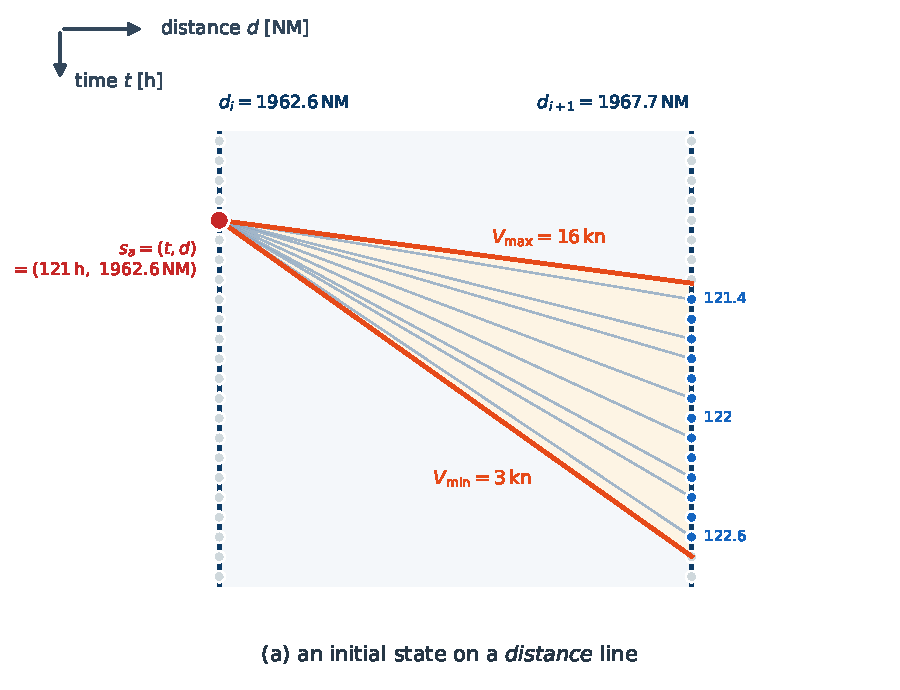
\includegraphics[width=\linewidth]{figures/state_neighbours.pdf}\par\vspace{2pt}
{\small (a) a state on a \emph{distance} line}
\end{minipage}\hfill
\begin{minipage}[t]{0.492\textwidth}
\centering
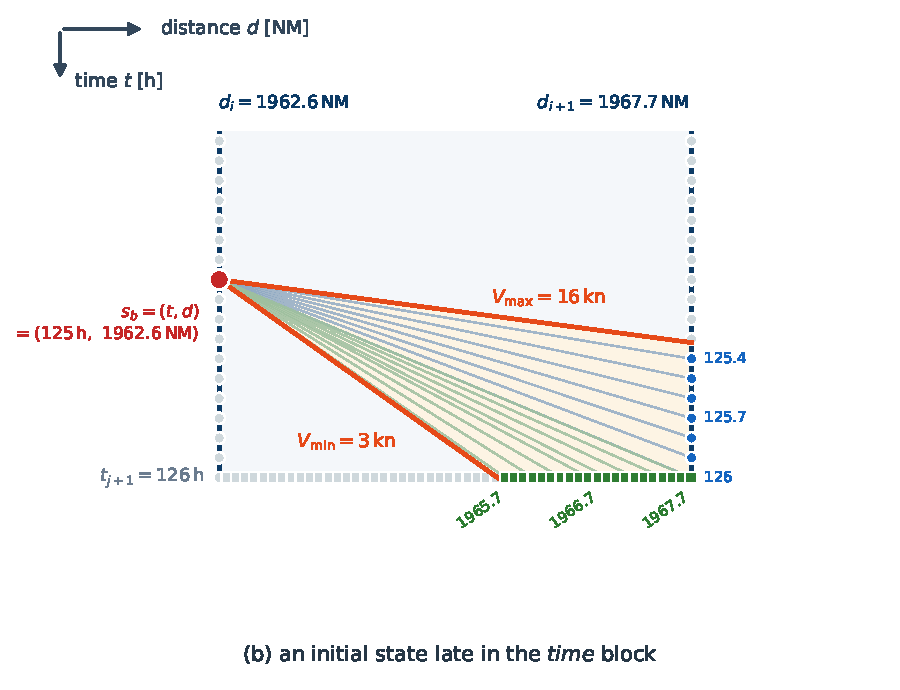
\includegraphics[width=\linewidth]{figures/state_neighbours_hline.pdf}\par\vspace{2pt}
{\small (b) a state on a \emph{time} line}
\end{minipage}
\caption{A state of the dynamic program and its candidate successors (values illustrative), for the
two cases of the grid --- the compass in each panel gives the reading: the horizontal axis is
distance $d$, increasing left to right; the vertical axis is elapsed time $t$, increasing top to
bottom. (a) the state sits on a \emph{distance} line --- the boundary it has just
crossed --- in the interior of a forecast block; (b) the state sits on a \emph{time} line --- a
decision epoch --- in the interior of a cell. In both cases every admissible speed leads to one of
two walls: the next distance line $d_{\mathcal{D}(d)}$, where the sea conditions change, or the
next time line $t_{\mathcal{T}(t)}$, where the forecast is refreshed. The speed cone
$\mathcal{V}=[0,v_{\max}]$ --- its slow edge vertical, $\bar v=0$: the vessel may wait in place ---
intersects the walls in two windows, and the grid picks out the nodes inside them: arrival times
spaced $\tau$ on the distance wall (circles) and arrival distances spaced $\delta$ on the time wall
(squares), the two families of Eq.~\eqref{eq:neighbors}. The fast edge of the cone crosses the
distance wall before the block ends, capping the second family; every slower speed, down to
waiting, runs out of the block first, clipping the first family at the time wall. Each surviving
node fixes its own leg speed $\bar v=(\tilde d-d)/(\tilde t-t)$, labelled on the grid in NM and
hours respectively.}
\label{fig:state-neighbours}
\end{figure}
When the vessel is streaming in a sub-segment that starts at point $d$ at time $t$  it is subject to the fixed sea conditions and with the same heading until the end of the sea condition time block and the end of the sub-segment, whatever it reaches first. I.e., it steams inside a given rectunglar area of the time--distance space demonstrated in Figure X.   Therefore, the FCR is determined only by $v$ within this rectunglar area.  We denote this FCR by $\phi(t, d; v)$ metric ton / hour.

The problem of minimizing the total fuel consumption of the voyage can be formulated as the following forward Bellman equation:


% ==== NEW (node-first: min over the neighbour set 𝒜; realised leg speed v̄ = Δd/Δt) ====
\begin{equation}
\label{eq:cost-to-arrive}
C^{*}(t,d)=\min_{\substack{(\tilde t,\tilde d) \in\mathcal{A}^{-1}( t, d)}}   \begin{cases}     \infty & \tilde t =  t_{\Theta} , d < d_M \\
	C^{*}(\tilde t,\tilde d)+(\tilde t- t)\,\phi(t,d; (\tilde d- d)/(\tilde t-t))  & \text{otherwise}
\end{cases}
\end{equation}
With the boundary condition $C^*(0,0) = 0$ and the the minimum total voyage fuel is obtained at $C^{*}(T,L)$.

We denote the solution of (\ref{eq:cost-to-arrive}) for each  state $(t,d)$ by  $(\tilde t^{\star},\tilde d^{\star})$. The value of this solution is
the minimum fuel to arrive on time at each state $(t,d)$ or infinity if it is not possible to meet the ETA. The SOG at the subsegment that starts at $(t,d)$ is
\begin{equation}
	\label{eq:opt-speed} V^{*}(t,d)= \frac{\tilde d^{\star} - d}{\tilde t^{\star} -t}
\end{equation}

% ==== NEW (node-first: realised speed of the optimal incoming leg) ====

%V^{*}(d,t)=\frac{d-\tilde d^{\star}}{t-\tilde t^{\star}},\qquad
%(\tilde d^{\star},\tilde t^{\star})=\arg\min_{\substack{(\tilde d,\tilde t)\in\mathcal{S}\,:\,(d,t)\in\mathcal{A}(\tilde d,\tilde t)\\ (d-\tilde d)/(t-\tilde t)\,\in\,\mathcal{V}}}
%\Bigl[\, C^{*}(\tilde d,\tilde t)+(t-\tilde t)\,\phi\bigl(\tilde d,\tilde t;\tfrac{d-\tilde d}{t-\tilde t}\bigr)\,\Bigr].



% ==== NEW (2026-08-06, approved in the Aug-5 meeting — item 1C): the shortest-path reading, as a bridge into §4.2.
% ==== Direction-neutral wording (C* semantics left to Eq. 6 / Algorithm 1, pending Tal's direction reconciliation) ====
The states and their successor sets give the problem a compact graph reading: the states of
$\mathcal{S}$ are the vertices of a directed graph, and each admissible leg
$(t,d)\to(\tilde t,\tilde d)$ with $(\tilde t,\tilde d)\in\mathcal{A}(t,d)$ is an arc weighted by
its leg fuel, $(\tilde t-t)\,\phi(t,d;(\tilde d-d)/(\tilde t-t))$. Minimising the voyage fuel
subject to the ETA is then a \emph{shortest-path problem} on this graph: the minimum voyage fuel is
the shortest distance from $(0,0)$ to the destination, and the optimal speed schedule \emph{is} the
shortest path itself --- each of its arcs read as a leg sailed at the slope
$(\tilde d-d)/(\tilde t-t)$. Because every arc strictly increases time, the graph is acyclic, so the
shortest path requires no label-correcting method; the next section computes it in a single forward
pass.

\subsection{Solving the Bellman equation}
\label{sec:solve}
% ==== labels of the former subsections (removed in the 2026-08-04 flat rewrite) kept so no \ref dangles ====
\label{sec:snap}\label{sec:enumerate}\label{sec:sweep}\label{sec:extract}\label{sec:tractability}


% ==== OLD (predecessor / incoming / back-tracking — wording predates the cost-to-go flip; its own formula was already outgoing) — superseded; kept, not rendered ====
%for each state we record the minimising predecessor and the realised leg speed $\bar v= (\tilde d- d)/(\tilde t-t)$ of the incoming arc, from which the optimal speed schedule is recovered by back-tracking to the origin.
% ==== OLD (standalone recovery sentence — its content is absorbed into the intro below and Stages 2-3; 2026-08-04 restructure) ====
%For each state we record the minimising successor $(\tilde d^{\star},\tilde t^{\star})$ and the realised leg speed $\bar v=(\tilde d^{\star}- d)/(\tilde t^{\star}-t)$ of the outgoing arc, from which the optimal speed schedule is recovered by walking forward from the origin.


% ==== OLD (S had to be "made finite" — written before §4.1 defined the explicit grid) — superseded; kept, not rendered ====
\begin{comment}
Equation~\eqref{eq:cost-to-arrive} defines the cost-to-arrive at any reachable state, but two things
must be settled before it can be evaluated. First, the state set $\mathcal{S}$ of
Eq.~\eqref{eq:state-space} has to be made not merely finite but of tractable size. Second, $\mathcal{S}$
and the speed transitions between its states have to be enumerated so the recursion can be swept. We
address discretisation first, then give the enumeration and the sweep as pseudocode.
\end{comment}
% ==== OLD ("Three things remain: bound, enumerate, sweep" — organized around the old two-algorithm split) ====
% ==== superseded by the stage-mirrored walkthrough (2026-08-04 restructure); kept, not rendered ====
\begin{comment}
Equations~\eqref{eq:state-space} and~\eqref{eq:neighbors} already define the state grid $\mathcal{S}$
and, for every state, its admissible successors $\mathcal{A}(d,t)$; the recursion of
Eq.~\eqref{eq:cost-to-arrive} is therefore well posed on a finite graph. Three things remain before it
can be evaluated efficiently. First, to bound the size of $\mathcal{S}$ and of the induced arc set.
Second, to enumerate --- out of the full grid --- only the states actually \emph{reachable} from the
origin and only the arcs whose realised speed is admissible, since these are typically a small
fraction of the whole. Third, to sweep the recursion over the resulting graph. We bound first, then
give the enumeration, the backward sweep, and the schedule extraction as a single pseudocode
(Algorithm~1).
\end{comment}
% ==== OLD intro (subsection-roadmap version, referenced §4.2.1-4.2.3) — superseded by the flat rewrite (2026-08-04); kept, not rendered ====
\begin{comment}
Section~\ref{sec:states} supplies every mathematical object the solution requires: the state grid
$\mathcal{S}$ (Eq.~\eqref{eq:state-space}), the successor set $\mathcal{A}(d,t)$ of each state
(Eq.~\eqref{eq:neighbors}), the fuel-to-go recursion that couples them
(Eq.~\eqref{eq:cost-to-arrive}) with its boundary condition, and the optimal outgoing speed
(Eq.~\eqref{eq:opt-speed}). What remains is computational: the recursion must be evaluated exactly
once per state, over only the reachable part of the grid, in an order that makes every evaluation
final. Algorithm~1 organises this into three stages, each answering one question a reader arriving
from Section~\ref{sec:states} would ask. Stage~1 (\emph{forward closure},
Section~\ref{sec:enumerate}) asks \emph{which decisions exist}: starting from $(0,0)$ it discovers
the reachable states and, for each, materialises the successor set $\mathcal{A}(d,t)$ as arcs priced
with the fuel term of Eq.~\eqref{eq:cost-to-arrive} --- building the graph is precisely the
calculation the backpropagation needs. Stage~2 (\emph{backpropagation}, Section~\ref{sec:sweep})
asks \emph{what each decision costs from there to the destination}: it evaluates
Eq.~\eqref{eq:cost-to-arrive} once per state, in an order that guarantees every successor is already
valued, recording the minimising successor. Stage~3 (\emph{extraction}, Section~\ref{sec:extract})
asks \emph{which decisions to take}: two closing lines read the optimal fuel at the origin and
unroll the speed schedule by walking forward along the recorded successors. The pseudocode
introduces no new mathematics --- every line evaluates an object already defined in
Section~\ref{sec:states}; what the algorithm adds is the \emph{order} of evaluation. Line numbers
are referenced throughout the walkthrough below.
\end{comment}
% ==== OLD (2026-08-04 flat rewrite: build+price in one pass, then one BACKWARD sweep) — superseded by Tal's
% ==== Aug-5 algorithm (forward one-pass relaxation + backtrack extraction); kept, not rendered ====
\begin{comment}
Section~\ref{sec:states} supplies every mathematical object the solution requires: the state grid
$\mathcal{S}$ (Eq.~\eqref{eq:state-space}), the successor set $\mathcal{A}(d,t)$ of each state
(Eq.~\eqref{eq:neighbors}), the fuel-to-go recursion that couples them
(Eq.~\eqref{eq:cost-to-arrive}) with its boundary condition, and the optimal outgoing speed
(Eq.~\eqref{eq:opt-speed}). What remains is computational, and it is organised around one design
decision. Discovering the reachable states, placing them on the discrete grid, and computing the FCR
price of every arc are not three steps but \emph{one}: a single forward pass (lines~1--10 of
Algorithm~1) enumerates, from each state, only the grid nodes actually reachable within
$\mathcal{V}$ --- and each node it emits arrives already discretised, already carrying its leg speed
$\bar v=(\tilde d-d)/(\tilde t-t)$, and already priced at $\phi(d,t;\bar v)\,(\tilde t-t)$, the fuel
term of Eq.~\eqref{eq:cost-to-arrive}. This is the optimised graph construction: when the pass ends,
the graph is not merely built --- it is fully priced, and the expensive physics (one
still-water-speed inversion and FCR evaluation per arc) has been paid exactly once per arc. Solving
the problem then costs a single \emph{backward} sweep (lines~11--14): one evaluation of
Eq.~\eqref{eq:cost-to-arrive} per state, in an order that guarantees every successor is already
valued, yielding the optimal outgoing speed of \emph{every} reachable state --- a full policy, not
one path. Two closing lines (15--16) read the optimal fuel at the origin and unroll the speed
schedule. The pseudocode introduces no new mathematics --- every line evaluates an object already
defined in Section~\ref{sec:states}; the walkthrough below follows its line numbers.
\end{comment}
% ==== NEW (2026-08-06: matched to Tal's Aug-5 Algorithm 1 — ONE forward pass does discovery, discretisation,
% ==== pricing AND valuation; only the winning predecessor is stored; extraction backtracks from the terminal state) ====
Section~\ref{sec:states} supplies every mathematical object the solution requires: the state grid
$\mathcal{S}$ (Eq.~\eqref{eq:state-space}), the successor set $\mathcal{A}(t,d)$ of each state
(Eq.~\eqref{eq:neighbors}), the Bellman recursion that couples them
(Eq.~\eqref{eq:cost-to-arrive}), and the optimal leg speed (Eq.~\eqref{eq:opt-speed}). What remains
is computational, and it is organised in two main loops. The first loop, discovers the reachable states,
places them on the discrete grid, prices every leg, and calculate the \emph{value} of every state.  All of these are preformed in a single forward pass (lines~1--9 of Algorithm~1) processes the states in
lexicographic $(t,d)$ order.
For each state $(t,d)$  the algorithm scans the discretized reachable states $(\tilde t, \tilde d)  \in \mathcal{A}(t,d)$.
Each candidate state arrives already discretised. The leg speed
$\bar v=(\tilde d-d)/(\tilde t-t)$ implied by the state transition and priced on the spot at $\phi(t,d;\bar v)\,(\tilde t-t)$. The value of the endpoint $(\tilde t, \tilde d)$ is
immediately updated  (lines~6--7). For each state the aglrithm stores its value $C^{*}$ and its winning predecessor
$pred(\cdot)$ (line~8). The actual arc set is not stored yet the expensive physics of the FCR evaluation per leg is peformed exactly once, when the leg's source
is expanded. Because every leg strictly increases time, the lexicographic scan order guarantees that
a state's value is final before the state is expanded.
Extraction of the actual journeyis then preformed (lines~10--15).  The voyage terminates at $(T,L)$, possibly with some waiting at distance $L$ so an early arrival continues to the deadline at
zero speed. The optimal journey $J^{\star}$ is read by backtracking the recorded
predecessors to the origin.

% ==== Algorithm 1 box (moved up from after the enumeration prose, 2026-08-04 restructure: box first, walkthrough after) ====
\begin{center}
\fbox{\begin{minipage}{0.95\textwidth}
\textbf{Algorithm~1: Solve the Bellman's equations}\\[-6pt]
\rule{\linewidth}{0.4pt}
\footnotesize
\begin{tabbing}
xxx\=xx\=xx\=xx\=xxxxxxxxxxxxxxxxxxxxxxxxxxxxxx\=\kill
\textbf{Input:} distance lines $d_0<\dots<d_M{=}L$, time lines $t_0<\dots<t_\Theta{=}T$, speed band $[0,v_{\max}]$, snaps $\delta,\tau$, FCR $\phi$\\
\textbf{Output:}  Speed schedule and total fuel consumption \\
{\small$\triangleright$ \emph{Stage 1 --- forward closure: discover all reachable states and calculate their values}}\\
{\scriptsize 1}\> $C^*(0,0) \leftarrow 0$; \quad $C^*(t,d) \leftarrow \infty$ \, for all $(t,d) \ne (0,0)$;\\
{\scriptsize 2}\>  Define priority queue $Q\leftarrow[(0,0)]$\\
{\scriptsize 3}\> \textbf{while} $Q$ not empty \textbf{do}\\
{\scriptsize 4}\>\> $(t,d)\leftarrow \mathrm{pop}(Q)$ minimal element lexicograpgically;\\
{\scriptsize 5}\>\> \textbf{for} $(\tilde t,\tilde d)\in \mathcal{A}(t,d)$ \textbf{do}    \quad{\small$\triangleright$ scan all reachable states, see \eqref{eq:neighbors}} \\
%{\scriptsize 6}\>\>\> $\bar v\leftarrow(\tilde d-d)/(\tilde t-t)$;\quad \textbf{if} $\bar v$ unattainable at $(d,t)$ \textbf{then continue}\\
%{\scriptsize 7}\>\>\> $\mathcal{A}\leftarrow\mathcal{A}\cup\bigl\{\,(d,t)\!\to\!(\tilde d,\tilde t)\ \text{with speed}\ \bar v,\ \text{cost}\ \phi(d,t;\bar v)\,(\tilde t-t)\,\bigr\}$\\
{\scriptsize 6}\>\>\> \textbf{if} $C^*(t,d)+ \phi(t,d;(\tilde d-d)/(\tilde t-t))\,(\tilde t-t)< C^{*}(\tilde t,\tilde d)$ \textbf{then} \\
{\scriptsize 7}\>\>\>\> $C^{*}(\tilde t,\tilde d) \leftarrow C^*(t,d)+ \phi(t,d;(\tilde d-d)/(\tilde t-t))\,(\tilde t-t)$; \quad{\small$\triangleright$ update state value, see \eqref{eq:cost-to-arrive}}\\
{\scriptsize 8}\>\>\>\> $pred(\tilde t,\tilde d) \leftarrow (t,d)$; \\
{\scriptsize 9}\>\>\> \textbf{if} $(t,d) \notin Q$ then $push(Q,(t,d))$; \\
{\small$\triangleright$ \emph{Stage 2 --- extraction}}\\
{\scriptsize 10}\> $curr \leftarrow (T,L)$; \\
{\scriptsize 11}\> $J^{\star} \leftarrow [curr]$; \\
{\scriptsize 12}\> \textbf{while} $curr \ne (0,0)$ \textbf{do}\\
{\scriptsize 13}\>\> $curr \leftarrow pred(curr)$ ;\\
 {\scriptsize 14}\>\> $J^{\star} \leftarrow [curr] + J^{\star}$; \\
{\scriptsize 15}\> \textbf{return}  $J^{\star}$ (optimal journey) 
\end{tabbing}
\end{minipage}}
\end{center}




%% ============================================================ 5. DATA & EXPERIMENTAL DESIGN
\section{Data and experimental design}
\label{sec:data}
In this section we describe the testbed on which the method of Section~\ref{sec:methods} is evaluated.
We first present the data that define the problem instances --- the sea conditions queried along each
route and the voyages themselves --- and then the experimental design: the settings under which the
dynamic program is exercised and the baselines against which it is compared, namely a fixed-speed
operational reference and the state-of-the-art block formulation of \citet{luo2024}.

\subsection{Data}

\subsubsection{Sea conditions data}
The sea conditions were obtained from the Open-Meteo API \citep{openmeteo}, which redistributes the
outputs of operational \emph{numerical weather prediction} (NWP) models --- physics-based forecasting
systems that integrate the governing equations of the atmosphere and ocean forward in time from an
estimated initial state, and that periodically re-initialise on a fixed cycle. One product was used
per environmental driver:
\begin{itemize}
\item \textbf{Wind} (10 m speed and direction) --- the NOAA \emph{Global Forecast System} (GFS), the
operational global atmospheric model of the U.S.\ weather service, at $0.25\degree$ resolution,
re-initialised every 6 h (at 00/06/12/18 UTC) and forecasting to a 168 h horizon.
\item \textbf{Waves} (significant wave height) --- the M\'et\'eo-France wave model (MFWAM), a
third-generation spectral ocean-wave model, at $0.25\degree$ resolution, re-initialised twice daily,
to 168 h.
\item \textbf{Ocean currents} (velocity and direction) --- the M\'et\'eo-France SMOC ocean model, at
$0.08\degree$ resolution, re-initialised once daily, to 168 h.
\end{itemize}
The Beaufort number consumed by the speed model was computed from the 10 m wind speed rather than
read from the API (Section~\ref{sec:problem}). For each route, two records were collected at every
waypoint on a 6 h sampling cadence over $\sim$80 days and stored in HDF5 with separate tables: the
\emph{actual} weather --- the conditions ultimately realised --- and the \emph{predicted} weather ---
every forecast cycle issued ahead of those conditions. The actual record provides the ground-truth
conditions against which a voyage is evaluated; the predicted record provides the forecasts available
to a planner at each decision point.

\paragraph{Forecast accuracy.} The two records also let forecast error be quantified directly, by
comparing each predicted value against the actual weather later observed at the same waypoint and
time, as a function of lead time. Wind-speed RMSE grew systematically with lead time: it approximately
doubled over the first 133 h on the milder route (4.13 $\rightarrow$ 8.40 km/h) and grew more steeply
on the harsher one ($+286\%$ over 144 h) \todo{FIG: forecast error vs lead time}. This degradation is
an intrinsic property of the data, reported here independent of any optimisation; it is why a
rolling-horizon plan, which commits speeds against forecasts that are later revised, consumes more
fuel than a perfect-foresight oracle (Section~\ref{sec:res-rh}).

\paragraph{NWP model refresh cycle.} Each product refreshes on its own fixed cycle, which sets the
re-plan cadence used later. The GFS wind product refreshes every 6 h, MFWAM (waves) every 12 h, and
SMOC (currents) every 24 h. The predicted-weather record confirms this: at a 1 h query cadence, 86\%
of consecutive wind values were identical to the previous hour (94\% for waves, 97\% for currents).
Re-planning more frequently than 6 h therefore acts on no new wind information, which is why the 6 h
cadence used below is set by the data rather than tuned.

\subsubsection{Voyage data}
%Each voyage is a fixed route of total length $L$ to be completed within a required arrival time $T$
Two routes were used to benchmark our algoritm:
\begin{enumerate}
	\item   \emph{Indian Ocean} route (Persian Gulf $\rightarrow$ Strait of Malacca). This is a 3,393 NM long route that crosses a  calm stretch of ocean with  relatively stable conditions.
	\item  \emph{North Atlantic} route (St.~John's $\rightarrow$ Liverpool). This is s shorter route (1,955 NM), with rougher and more volotile sea conditions.
\end{enumerate} chosen to contrast weather regimes: Route~1
The two routes are depicte in Figure~\ref{fig:routes} and their waypoints are detailed in Table~\ref{tab:waypoints}.  The speed optimization problem can be solved with various ETA values. Moreover, because the sea conditions changes over time, a problem instance is determined by the  route, departure time and desired ETA.  In our experiment we tseted each route with 25 different depature times during the spring of 2026, spaced three days appart.  Each of these $2 \times 25$ route-departure times combinations were teseted with 3 ETA levels corrosponding to an average sailing speed of 10, 12, and 14 NM, making a benchmark set consisting of 150 problem instances. 

\begin{figure}[ht]
\centering
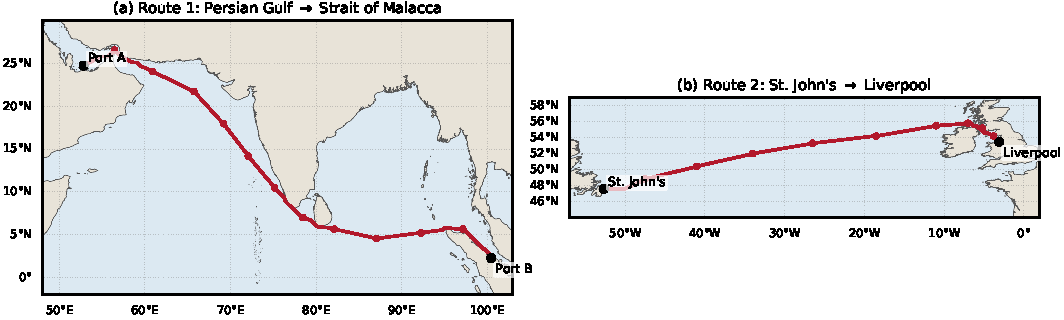
\includegraphics[width=\textwidth]{figures/routes.pdf}
\caption{The two study routes and their waypoints: (a) Route~1, Persian Gulf $\rightarrow$ Strait of
Malacca; (b) Route~2, St.\ John's $\rightarrow$ Liverpool (North Atlantic).}
\label{fig:routes}
\end{figure}

\begin{table}[ht]
\centering
\footnotesize
\caption{Waypoints of the two routes (decimal degrees; positive north / east).}
\label{tab:waypoints}
\begin{tabular}{rlrr@{\hspace{1.5em}}rlrr}
\toprule
\multicolumn{4}{c}{Route 1: Persian Gulf $\rightarrow$ Strait of Malacca (3{,}393 nm)} &
\multicolumn{4}{c}{Route 2: St.\ John's $\rightarrow$ Liverpool (1{,}955 nm)} \\
\cmidrule(lr){1-4}\cmidrule(lr){5-8}
\# & Waypoint & Lat & Lon & \# & Waypoint & Lat & Lon \\
\midrule
1  & Port A (Persian Gulf)       & 24.75 & 52.83  & 1  & St.\ John's          & 47.57 & $-52.71$ \\
2  & Gulf of Oman                & 26.55 & 56.45  & 2  & Grand Banks          & 48.80 & $-47.50$ \\
3  & Arabian Sea 1               & 24.08 & 60.88  & 3  & Mid-Atlantic West    & 50.40 & $-41.00$ \\
4  & Arabian Sea 2               & 21.73 & 65.73  & 4  & Mid-Atlantic Central & 52.00 & $-34.00$ \\
5  & Arabian Sea 3               & 17.96 & 69.19  & 5  & Mid-Atlantic East    & 53.30 & $-26.50$ \\
6  & Arabian Sea 4               & 14.18 & 72.07  & 6  & Rockall Bank         & 54.20 & $-18.50$ \\
7  & Indian Ocean 1              & 10.45 & 75.16  & 7  & West of Ireland      & 55.50 & $-11.00$ \\
8  & Indian Ocean 2              &  7.00 & 78.46  & 8  & Malin Head           & 55.80 & $-7.00$  \\
9  & Bay of Bengal               &  5.64 & 82.12  & 9  & North Channel        & 55.20 & $-5.20$  \\
10 & Indian Ocean 3              &  4.54 & 87.04  & 10 & Irish Sea North      & 54.20 & $-3.80$  \\
11 & Andaman Sea 1               &  5.20 & 92.27  & 11 & Liverpool            & 53.41 & $-3.01$  \\
12 & Andaman Sea 2               &  5.64 & 97.16  &    &                      &       &          \\
13 & Port B (Strait of Malacca)  &  1.81 & 100.10 &    &                      &       &          \\
\bottomrule
\end{tabular}
\end{table}

\subsection{Experimental design}
The deterministic dynamic program of Section~\ref{sec:methods} is exercised across two independent
axes: the \emph{granularity} of the speed decision and the \emph{information} available when the plan
% ==== OLD (common grid of 61 SOG values) — superseded by the band 𝒱; kept, not rendered ====
\begin{comment}
is made. Throughout, the speed search uses a common grid of 61 SOG values spanning the mean voyage
speed $L/T \pm 3$ kn, and the arrival time $T$ was binding in every run (zero slack) --- so all
comparisons are at equal voyage time, isolating the effect of the setting rather than the schedule's
duration.
\end{comment}
% ==== NEW (speed drawn from the band 𝒱; enumeration is node-first, §4.2) ====
is made. Throughout, the speed at each decision is drawn from a common band spanning the mean voyage
speed $L/T \pm 3$ kn --- the interval $\mathcal{V}$ of Section~\ref{sec:methods}, enumerated
node-first on the $\delta,\tau$ grid --- and the arrival time $T$ was binding in every run (zero slack)
--- so all comparisons are at equal voyage time, isolating the effect of the setting rather than the
schedule's duration.

\subsubsection{Speed-decision granularity}
\textbf{SR (this paper).} The method under test is the dynamic program of Section~\ref{sec:methods} applied
without restriction: the speed is re-chosen at every boundary crossing, so the plan adapts to each
change of heading or sea conditions along the route.

\noindent\textbf{Luo (2024).} The state-of-the-art baseline of \citet{luo2024}
restricts the speed to be constant within each time block. Its graph is a lattice of (column,
distance) nodes, where columns mark times $0,\Delta t,2\Delta t,\dots$; each arc spans one block and
is traversed at a single constant SOG equal to the block distance divided by $\Delta t$. The arc cost
is obtained by walking the weather sub-segments within the block and summing fuel at that fixed block
SOG, and the minimum-fuel path to the ETA column is found by shortest path. The defining restriction
is that speed cannot vary in response to weather that changes inside a block. This baseline was
implemented independently from its published description --- with its own lattice and arc evaluation,
not as SR subject to an added equality constraint --- so the comparison reflects
Luo's actual method rather than a weakened variant. Any fuel difference from SR is
therefore attributable to decision granularity alone.

\noindent\textbf{Fixed-speed (Naive).} The operational reference is a set-and-forget policy that
sails a single fixed mean SOG ($L/T$) through the actual time-varying weather, with no optimisation
and no re-planning.

\subsubsection{Information regime}
\textbf{Perfect foresight (oracle).} Each leg is evaluated against the actual weather recorded at the
voyage's departure sample hour, giving the planner perfect knowledge of conditions. This bounds the
achievable advantage (Section~\ref{sec:res-oracle}).

\noindent\textbf{Rolling horizon.} The planner is re-solved at 6 h decision steps. At each step the
first 6 h block is planned against actual (nowcast) weather and the remainder against the most recent
available predicted cycle; only the first block is committed before advancing and re-planning.
Realised fuel is the sum of the committed blocks. The 6 h cadence equals the GFS NWP cycle (above).
Both SR and Luo are exercised under this regime.

\subsubsection{Evaluation protocol}
\label{sec:protocol}
Each route was evaluated as a \emph{consecutive-voyage chain} in which voyage $N{+}1$ departs at the
sample hour at which voyage $N$ arrives. Fixing the step to the ETA guaranteed that every planner
encountered identical departure weather at every voyage. Under perfect foresight, thirteen voyages were
run on Route~1 and twenty-two on Route~2 --- 35 in total --- spanning the full collection window to
date ($\sim$155 days). Rolling-horizon evaluation currently covers the original 19-voyage subset (seven
on Route~1, twelve on Route~2 --- the first $\sim$80 days of the same chain); extending it to the full
35 is left to future work (Section~\ref{sec:limitations}). At each departure SR and Luo were run under
the perfect-foresight oracle and, on the 19-voyage subset, the 6 h rolling horizon, with the
rolling-horizon result compared against the Naive baseline. Because identical departure weather was
presented to all planners, the reported differences are attributable to the experimental setting ---
decision granularity and information regime --- not to sampling.

%% ============================================================ 7. RESULTS
\section{Results}
\label{sec:results}
Throughout, SR denotes the Shafir--Raviv per-leg free-speed dynamic program and Luo the per-block
speed-locked formulation of \citet{luo2024}.

\subsection{Fuel under perfect foresight}
\label{sec:res-oracle}
We evaluated 35 voyages, 13 on Route~1 and 22 on Route~2, spanning the full collection window to date
($\sim$155 days). In every voyage both SR and Luo consumed the full time budget (zero arrival slack).
We also report Naive, the fixed mean-SOG policy of Section~\ref{sec:methods} sailed through the same
actual weather, as a third reference point. Per-voyage fuel is reported in Tables~\ref{tab:modec-r1}
and~\ref{tab:modec-r2}; aggregates are in Table~\ref{tab:modec}.

\begin{table}[ht]
\centering
\tiny
\caption{Perfect-foresight aggregates (35 voyages). Naive is the fixed mean-SOG constant speed under
the same actual weather. Spread is a 95\% paired bootstrap CI (a paired $t$-interval cross-check
agreed closely throughout, not shown); negative gap = the first method burns less fuel.}
\label{tab:modec}
\begin{tabular}{lrrrrrrr}
\toprule
Route & $n$ & SR (mt) & Luo (mt) & Naive (mt) & SR$-$Luo (\%) & SR$-$Naive (\%) & Luo$-$Naive (\%) \\
\midrule
1 (Malacca)  & 13 & 346.48 [341.6, 351.4] & 352.84 [347.7, 358.1] & 355.07 [349.7, 360.6] & $-1.80$ [$-2.10,-1.50$] & $-2.41$ [$-2.71,-2.12$] & $-0.62$ [$-0.74,-0.51$] \\
2 (Atlantic) & 22 & 196.75 [192.1, 201.8] & 202.01 [197.2, 207.2] & 203.88 [198.9, 209.3] & $-2.60$ [$-2.89,-2.31$] & $-3.48$ [$-3.80,-3.14$] & $-0.91$ [$-1.05,-0.76$] \\
\bottomrule
\end{tabular}
\end{table}

\begin{table}[ht]
\centering
\caption{Perfect-foresight per-voyage fuel, Route 1 (Malacca, ETA 280 h). $\mathrm{sh}_0$ = departure
sample hour. Negative gap = SR burns less fuel than Luo.}
\label{tab:modec-r1}
\begin{tabular}{
  S[table-format=2.0]
  S[table-format=4.0]
  S[table-format=3.2]
  S[table-format=3.2]
  S[table-format=3.2]
  S[table-format=-1.2]
}
\toprule
{Voyage} & {$\mathrm{sh}_0$} & {SR (mt)} & {Luo (mt)} & {Naive (mt)} & {SR$-$Luo (\%)} \\
\midrule
1  & 6    & 354.91 & 361.67 & 362.74 & -1.87 \\
2  & 286  & 355.23 & 364.68 & 367.03 & -2.59 \\
3  & 566  & 338.25 & 343.32 & 345.42 & -1.48 \\
4  & 846  & 348.53 & 353.30 & 354.74 & -1.35 \\
5  & 1126 & 337.61 & 340.89 & 342.68 & -0.96 \\
6  & 1406 & 335.23 & 344.18 & 346.19 & -2.60 \\
7  & 1686 & 347.23 & 353.32 & 356.03 & -1.72 \\
8  & 1966 & 331.99 & 339.19 & 340.29 & -2.12 \\
9  & 2246 & 339.48 & 343.81 & 346.05 & -1.26 \\
10 & 2526 & 349.29 & 355.70 & 358.69 & -1.80 \\
11 & 2806 & 356.37 & 366.29 & 368.50 & -2.71 \\
12 & 3086 & 347.89 & 354.20 & 356.87 & -1.78 \\
13 & 3366 & 362.26 & 366.40 & 370.62 & -1.13 \\
\bottomrule
\end{tabular}
\end{table}

\begin{table}[ht]
\centering
\caption{Perfect-foresight per-voyage fuel, Route 2 (Atlantic, ETA 168 h). $\mathrm{sh}_0$ = departure
sample hour. Negative gap = SR burns less fuel than Luo.}
\label{tab:modec-r2}
\begin{tabular}{
  S[table-format=2.0]
  S[table-format=4.0]
  S[table-format=3.2]
  S[table-format=3.2]
  S[table-format=3.2]
  S[table-format=-1.2]
}
\toprule
{Voyage} & {$\mathrm{sh}_0$} & {SR (mt)} & {Luo (mt)} & {Naive (mt)} & {SR$-$Luo (\%)} \\
\midrule
1  & 0    & 203.36 & 210.48 & 212.61 & -3.38 \\
2  & 168  & 204.24 & 209.52 & 212.78 & -2.52 \\
3  & 336  & 197.05 & 202.78 & 203.65 & -2.82 \\
4  & 504  & 206.33 & 212.69 & 214.54 & -2.99 \\
5  & 672  & 216.28 & 223.58 & 225.98 & -3.26 \\
6  & 840  & 190.73 & 197.30 & 200.50 & -3.33 \\
7  & 1008 & 227.91 & 233.82 & 237.09 & -2.53 \\
8  & 1176 & 194.46 & 198.31 & 200.43 & -1.95 \\
9  & 1344 & 195.83 & 198.53 & 199.35 & -1.36 \\
10 & 1512 & 193.11 & 197.17 & 198.99 & -2.06 \\
11 & 1680 & 199.51 & 204.09 & 206.86 & -2.25 \\
12 & 1848 & 198.93 & 204.79 & 206.10 & -2.86 \\
13 & 2016 & 214.21 & 220.09 & 222.48 & -2.67 \\
14 & 2184 & 185.26 & 190.53 & 192.45 & -2.76 \\
15 & 2352 & 186.96 & 190.85 & 191.62 & -2.04 \\
16 & 2520 & 193.81 & 200.40 & 201.60 & -3.29 \\
17 & 2688 & 179.34 & 187.47 & 188.51 & -4.33 \\
18 & 2856 & 178.68 & 183.26 & 185.41 & -2.50 \\
19 & 3024 & 190.52 & 196.15 & 197.61 & -2.87 \\
20 & 3192 & 188.98 & 192.51 & 194.09 & -1.83 \\
21 & 3360 & 188.62 & 193.37 & 194.52 & -2.45 \\
22 & 3528 & 194.27 & 196.57 & 198.10 & -1.17 \\
\bottomrule
\end{tabular}
\end{table}

\noindent\textbf{SR consumed less fuel than Luo on every voyage.} SR was more fuel-efficient on all 35
of 35 voyages, with no exception on either route. The per-voyage advantage ranged from 3.28 to 9.92 mt
on Route~1 and from 2.30 to 8.12 mt on Route~2.

\noindent\textbf{The absolute advantage was comparable across routes, but proportionally larger on
the shorter voyage.} The mean saving was similar in absolute terms: 6.36 mt on Route~1 and 5.27 mt on
Route~2, even though Route~2 takes roughly half the time. As a fraction of total fuel, the advantage is
therefore larger on the shorter, harsher Atlantic route (2.60\%) than on Malacca (1.80\%); the 95\% CIs
in Table~\ref{tab:modec} do not overlap. This is the scaling we expect from the convexity of fuel
consumption in speed (Section~\ref{sec:problem}).

\noindent\textbf{Both SR and Luo also beat Naive, with SR by the larger margin.} SR saved 2.41\% of
fuel relative to Naive on Route~1 and 3.48\% on Route~2. Luo's saving relative to Naive was smaller,
0.62\% and 0.91\%. This is because Luo can change its speed only once per block, while SR can change
it on every leg.

\noindent\textbf{Departure weather dominated voyage-to-voyage fuel variation.} On Route~2, under the
same formulation, the worst departure (227.91 mt) consumed 27.5\% more fuel than the best (178.68 mt).
This spread is far larger than the entire SR--Luo gap. The Atlantic fuel spread (27.6\%) was about
three times that of Malacca (9.1\%).

\subsection{Fuel under rolling-horizon planning (real forecasts)}
\label{sec:res-rh}
To test whether the advantage survives realistic operation, SR and Luo were embedded in the
6 h rolling-horizon scheme (Section~\ref{sec:protocol}) and compared against the Naive set-and-forget
baseline, over the original 19-voyage subset of the full chain (Section~\ref{sec:protocol}). Realised
fuel relative to Naive is reported per voyage in Tables~\ref{tab:rh-r1} and~\ref{tab:rh-r2} and
summarised in Table~\ref{tab:rh}.

\begin{table}[ht]
\centering
\caption{Rolling-horizon realised fuel relative to the Naive set-and-forget baseline.}
\label{tab:rh}
\begin{tabular}{lrrrr}
\toprule
Route & $n$ & RH-SR vs Naive (mean \%) & RH-Luo vs Naive (mean \%) & RH-SR saves on \\
\midrule
2 (Atlantic) & 12 & $-1.8$ & $0.0$  & 11/12 \\
1 (Malacca)  & 7  & $-1.3$ & $-0.0$ & 6/7 \\
\bottomrule
\end{tabular}
\end{table}

\begin{table}[ht]
\centering
\caption{Rolling-horizon per-voyage realised fuel, Route 1 (Malacca, ETA 280 h). $\mathrm{sh}_0$ =
departure sample hour. Negative \% = saving vs the Naive set-and-forget baseline.}
\label{tab:rh-r1}
\begin{tabular}{rrrrrr}
\toprule
$\mathrm{sh}_0$ & Naive (mt) & RH-SR (mt) & RH-Luo (mt) & RH-SR vs Naive (\%) & RH-Luo vs Naive (\%) \\
\midrule
6    & 362.64 & 357.37 & 362.57 & $-1.45$ & $-0.02$ \\
286  & 367.03 & 358.72 & 367.72 & $-2.27$ & $+0.19$ \\
566  & 344.58 & 344.91 & 344.51 & $+0.10$ & $-0.02$ \\
846  & 354.52 & 350.75 & 354.36 & $-1.06$ & $-0.05$ \\
1126 & 342.67 & 339.82 & 341.69 & $-0.83$ & $-0.29$ \\
1406 & 346.14 & 342.21 & 346.57 & $-1.14$ & $+0.12$ \\
1686 & 355.60 & 346.69 & 355.10 & $-2.50$ & $-0.14$ \\
\bottomrule
\end{tabular}
\end{table}

\begin{table}[ht]
\centering
\caption{Rolling-horizon per-voyage realised fuel, Route 2 (Atlantic, ETA 168 h). $\mathrm{sh}_0$ =
departure sample hour. Negative \% = saving vs the Naive set-and-forget baseline.}
\label{tab:rh-r2}
\begin{tabular}{rrrrrr}
\toprule
$\mathrm{sh}_0$ & Naive (mt) & RH-SR (mt) & RH-Luo (mt) & RH-SR vs Naive (\%) & RH-Luo vs Naive (\%) \\
\midrule
0    & 212.47 & 204.62 & 212.12 & $-3.69$ & $-0.16$ \\
168  & 212.32 & 210.17 & 211.41 & $-1.01$ & $-0.43$ \\
336  & 203.42 & 198.61 & 203.42 & $-2.36$ & $-0.00$ \\
504  & 214.49 & 213.48 & 216.01 & $-0.47$ & $+0.71$ \\
672  & 225.66 & 220.26 & 224.90 & $-2.39$ & $-0.33$ \\
840  & 200.19 & 193.81 & 199.04 & $-3.19$ & $-0.57$ \\
1008 & 237.01 & 232.47 & 235.33 & $-1.92$ & $-0.71$ \\
1176 & 200.22 & 196.75 & 200.71 & $-1.73$ & $+0.25$ \\
1344 & 197.83 & 198.61 & 200.49 & $+0.39$ & $+1.34$ \\
1512 & 198.27 & 195.20 & 198.28 & $-1.55$ & $+0.01$ \\
1680 & 206.25 & 202.00 & 205.70 & $-2.06$ & $-0.27$ \\
1848 & 205.82 & 202.99 & 206.27 & $-1.38$ & $+0.22$ \\
\bottomrule
\end{tabular}
\end{table}

\noindent\textbf{SR re-planning saved fuel; Luo re-planning did not.} Rolling-horizon
SR reduced realised fuel relative to set-and-forget on 17 of 19 voyages (mean $-1.8\%$ on Route~2,
$-1.3\%$ on Route~1; best $-3.69\%$). The two exceptions were marginal ($+0.10\%$ on Route~1,
$+0.39\%$ on Route~2), where committing early speeds against forecasts that were later revised cost
slightly more than holding the mean. Rolling-horizon Luo was statistically indistinguishable from
set-and-forget (mean within $0.05\%$ of Naive on both routes): its fixed block speed left no room to
exploit the refreshed forecasts. The SR--Luo contrast established under perfect foresight therefore
persisted under realistic, imperfect-forecast operation, on both routes and across the full departure
window.

\noindent\textbf{Realised fuel fell within the oracle--Naive envelope.} On every voyage the realised
RH fuel satisfied $\text{oracle}\le\text{RH}\le\text{Naive}$. Rolling-horizon SR sat between 1.3 and
8.0 mt above its oracle, the gap representing the cost of committing speeds against forecasts that
were subsequently revised.

\noindent\textbf{The two formulations re-planned differently.} A single-voyage diagnostic recorded how
often a refreshed forecast changed the committed first-block speed: rolling-horizon Luo revised on 17
of 27 re-plans (63\%), against 12 of 27 (44\%) for rolling-horizon SR --- yet those more frequent
adjustments yielded no net saving over set-and-forget, whereas SR's translated into the
fuel reductions above.

\subsection{Supporting observations}
Two measurements underpin the rolling-horizon design (Section~\ref{sec:data}). First, forecast
accuracy degraded systematically with lead time (wind RMSE roughly doubled over 133 h on Route~1;
$+286\%$ over 144 h on Route~2), establishing why realised RH fuel exceeded the oracle. Second, the
6 h re-plan cadence was fixed to the GFS model cycle, of which 86\% of hourly queries returned
identical data, so sub-6 h re-planning carried no new information.

%% ============================================================ 8. DISCUSSION
\section{Discussion}
\label{sec:discussion}

\subsection{Convexity predicted the result}
The result follows from a single structural property: the fuel-consumption rate is convex in speed
(Section~\ref{sec:problem}), so holding one speed across a block of varying weather forces the
still-water speed to vary and, by Jensen's inequality, wastes fuel relative to per-leg freedom. Two
qualitative predictions of this argument were borne out. First, the gap was signed and systematic:
under perfect foresight SR consumed less fuel than Luo on all 35 of 35 voyages --- the directional
signature of Jensen's inequality, not an average tendency. Second, the gap scaled with weather
variability: proportionally larger on the harsher Atlantic route (2.60\%) than on Malacca (1.80\%), as
expected for a penalty driven by within-block weather spread. The empirical magnitude --- roughly
6 mt per voyage --- is thus explained, not merely reported.

\subsection{Decision granularity, not data, is the limiting factor}
That the SR advantage persisted under realistic rolling-horizon operation
(Section~\ref{sec:res-rh}) confirms it is not an artefact of perfect information. A single-voyage
diagnostic makes the point concrete: Luo revised its committed first-block speed on
17 of 27 re-plans, against 12 of 27 for SR, yet only the latter's revisions turned
into fuel savings. Luo re-planned \emph{more} often under refreshed forecasts and
still gained less, because it lacked the within-block resolution to act on the new information --- it
can shift the single speed it holds over an entire stage, but cannot place a slower leg exactly where
and when the weather worsens. The limiting factor is therefore decision granularity, not data: better
information helps only a planner able to exploit it at the resolution at which the weather varies.

\subsection{When re-planning helps --- and when it does not}
\label{sec:disc-bound}
The rolling-horizon benefit over set-and-forget is real but bounded, and is not claimed to be
universal. On 2 of 19 voyages the SR RH plan consumed slightly more fuel than the Naive
baseline, and the Luo RH plan did so on several. The reason is the same convexity seen from the
other side: on near-uniform weather a constant speed is itself fuel-optimal, so any forecast-driven
speed variation can only add a Jensen penalty unless the weather-routing gain exceeds it. The value of
re-planning is therefore bounded by how much the weather actually varies over a departure's window ---
largest on variable departures, vanishing or reversing on calm ones. This is best read as a
savings-versus-departure relationship \todo{FIG: savings vs departure} rather than a single figure;
the relevant gate, stated precisely, is ``realised fuel $\le$ Naive'', satisfied by SR on 17 of 19
voyages and by Luo on a minority.

\subsection{Relation to prior work}
Our findings sharpen, rather than overturn, the established picture. The convexity of fuel in speed has
long been used to argue that a constant speed is optimal under uniform conditions \citep{Ronen2011,
Hvattum2013}; we use the same property from the other side --- under \emph{varying} conditions a
constant-speed or coarse-stage plan carries a systematic Jensen penalty --- and we measure it. Against
the state-of-the-art multistage-graph formulation of \citet{luo2024}, which holds speed constant across
each forecast-cycle stage to keep the $K^{N}$ profile space tractable, our contribution is twofold and
empirical: the per-cell resolution that stage-based formulations cannot reach without combinatorial
blow-up is obtained here in a single polynomial-time pass over a directed acyclic graph, and, on a
like-for-like comparison, that finer resolution is shown to \emph{pay} --- SR
consumed less fuel than \citet{luo2024} on all 35 voyages under perfect foresight, with the gap growing
with weather variability exactly as the convexity argument predicts.

The result also speaks to the forecast-uncertainty literature. Where earlier work established the value
of finer or adaptive planning only under perfect information, or represented uncertainty through
ensembles \citep{Vettor2022, Luo2023}, we drive the optimiser with real operational forecasts, assume
no probabilistic model of the forecast--realisation relationship, and tie the re-plan cadence to the
forecast refresh cycle rather than choosing it freely \citep{Tzortzis2021, Zheng2023}. Under this
regime the granularity advantage persists (17 of 19 voyages), and Luo's inability to
convert refreshed forecasts into savings --- despite re-planning more often --- isolates decision
granularity, not information, as the binding factor. Finally, in contrast to evaluations on constant or
synthetic weather, on single voyages, or under the simplification $V_s\!=\!V_g$ \citep{Cariou2011}, our
benchmark is driven by real sea-conditions data with an explicit still-water-to-ground speed correction
and SOG-targeted arrival, over many consecutive voyages on two contrasting routes.

\subsection{Limitations}
\label{sec:limitations}
(i) Two routes were studied; the route-length scaling of the gap is reported as a contrast, not a
curve. (ii) The arrival constraint was hard and binding (zero slack) throughout, so results describe
fuel at equal voyage time; relaxing the ETA is left to future work. (iii) The rolling-horizon nowcast
assumes the current 6 h block is observable; its realism depends on onboard sensing. (iv) Luo, though
implemented faithfully, is one of several possible block-locked formulations. (v) The perfect-foresight
comparison was extended to the full 35-voyage chain; the rolling-horizon comparison (Section~\ref{sec:res-rh})
still covers the original 19-voyage subset, and extending it to match is left to future work.

%% ============================================================ 9. CONCLUSION
\section{Conclusion}
\label{sec:conclusion}
This study compared SR (the Shafir--Raviv per-leg speed-freedom formulation) against Luo, the
per-block speed-locked formulation of \citet{luo2024}, for fuel-minimising ship routing under
time-varying weather, on two routes spanning two weather regimes.

Three conclusions follow. First, Luo's per-block speed-locking is fuel-suboptimal by a structural
mechanism: because the fuel-consumption rate is convex in still-water speed, holding one speed across a
block of varying weather forces inefficient speed excursions, and SR's per-leg freedom recovers the
loss (Jensen's inequality). Second, under perfect foresight SR's advantage was realised on every one
of 35 voyages --- comparable in absolute fuel across routes ($\sim$6 mt) but proportionally larger on
the shorter, harsher voyage. Third, the advantage survived realistic 6 h rolling-horizon operation
against real forecasts, on the 19-voyage subset evaluated to date: SR re-planning saved fuel relative
to set-and-forget on 17 of 19 voyages, whereas Luo re-planning did not, its value bounded by weather
variability.

The practical implication is that the resolution of the speed decision --- not the availability of
re-planning or fresh forecasts --- is the binding factor: Luo cannot convert better
information into fuel savings, while SR can. The expected saving can be anticipated
from the variability of the route's weather. Future work includes extending the rolling-horizon
comparison to the full 35-voyage chain, extending the route set to establish the route-length scaling
as a curve, relaxing the hard arrival constraint to a soft ETA penalty, and examining the sensitivity
of the conclusions to the fuel-speed exponent.

%% ============================================================ APPENDIX
\appendix

\section{Derivation of the fuel-consumption-rate function}
\label{app:fcr}

The optimisation takes the fuel-consumption-rate (FCR) function as an exogenous input
(Section~\ref{sec:problem}); its derivation is not a contribution of this paper. This appendix
documents how the cubic form used in Eq.~\eqref{eq:fcr} is obtained, following the method of
\citet{yang2020}, and states the assumptions under which it holds. The scope here is the
\emph{still-water} relation between FCR and still-water speed (SWS); the separate mapping from SWS to
speed over ground under weather is the speed-correction model summarised in Section~\ref{sec:sog}.

\subsection{The DTU--SDU power chain}
\label{app:fcr-chain}
\citet{yang2020} obtain FCR from a physical power chain based on the DTU--SDU resistance-and-propulsion
method of \citet{kristensen2012}, which provides empirical formulae for the resistance and efficiency
terms of container ships, bulk carriers and tankers. The representative oil-products tanker modelled
in this study has the principal particulars in Table~\ref{tab:ship}.

\begin{table}[ht]
\centering
\caption{Principal particulars of the representative oil-products tanker; resistance model and
coefficient tables from \citet{yang2020} and \citet{kristensen2012}.}
\label{tab:ship}
\begin{tabular}{lll}
\toprule
Parameter & Symbol & Value \\
\midrule
Length between perpendiculars & $L_{pp}$ & 200 m \\
Beam & $B$ & 32 m \\
Draft & --- & 12 m \\
Displacement & $\Delta$ & 50{,}000 t \\
Block coefficient & $C_b$ & 0.75 \\
Installed power & --- & 10{,}000 kW \\
Still-water speed range & $V_s$ & 11--13 kn \\
\bottomrule
\end{tabular}
\end{table}

For a vessel of known principal particulars and
payload sailing in still water at SWS $V_{sw}$ (in m/s), the total resistance is
\begin{equation}
\label{eq:app-rt}
R_T \;=\; \tfrac{1}{2}\,\rho\,S\,V_{sw}^{2}\,C_T ,
\end{equation}
where $\rho$ is the seawater density, $S$ the wetted surface, and $C_T$ the total resistance
coefficient, itself the sum of frictional, incremental, air and residual components,
\begin{equation}
\label{eq:app-ct}
C_T \;=\; C_F + C_A + C_{AA} + C_R .
\end{equation}
The effective (towing) power, the required brake power, and the FCR follow as
\begin{align}
P_E &\;=\; R_T\,V_{sw}, \label{eq:app-pe}\\
P_B &\;=\; P_E/\eta_T, \qquad \eta_T = \eta_H\,\eta_O\,\eta_R\,\eta_S, \label{eq:app-pb}\\
r   &\;=\; P_B\cdot \mathrm{SFOC}\cdot 10^{-6} \quad [\text{mt/h}], \label{eq:app-r}
\end{align}
where $\eta_T$ is the total propulsive efficiency (hull, open-water, relative-rotative and shaft
components) and $\mathrm{SFOC}$ is the specific fuel-oil consumption of the main engine (g/kWh), read
from the engine performance curve. The terms $S$, $C_F$, $C_A$, $C_{AA}$, $C_R$ and the four
efficiencies are computed from the empirical formulae of \citet{kristensen2012}; the resulting FCR is
evaluated at a range of SWS values.

\subsection{Reduction to the cubic form}
\label{app:fcr-cubic}
Substituting Eqs.~\eqref{eq:app-rt} and~\eqref{eq:app-pe} into~\eqref{eq:app-pb}--\eqref{eq:app-r}
gives
\begin{equation}
\label{eq:app-cubic}
r \;=\; \frac{\rho\,S\,C_T\,\mathrm{SFOC}}{2\,\eta_T}\,\cdot 10^{-6}\; V_{sw}^{3} .
\end{equation}
Over the narrow operating band of a commercial voyage (here roughly 8--16 kn), the resistance
coefficient $C_T$, the propulsive efficiency $\eta_T$ and the SFOC vary little with speed, so the
bracketed factor is effectively constant and FCR reduces to a cube law, $r = a\,V_s^{3}$. This is the
origin of the cubic dependence asserted in Eq.~\eqref{eq:fcr}; it is also why FCR is \emph{strictly
convex} in SWS, the structural property the paper exploits (Section~\ref{sec:methods}). The cube law
is the standard ``admiralty'' approximation and is consistent with the broader speed--power literature.

\subsection{Calibration of the coefficient}
\label{app:fcr-calib}
The constant $a$ is vessel-specific. For the representative tanker of this study
(Table~\ref{tab:ship}) we obtain the calibrated FCR
\begin{equation}
\label{eq:fcr}
\fcr(V_s) \;=\; 0.000706\, V_s^{3} \quad [\text{mt/h},\; V_s \text{ in kn}],
\end{equation}
calibrated against the measured fuel-consumption data reported by \citet{yang2020} for a tanker of
comparable class. \citet{yang2020} verify the fuel-consumption function against measured noon-report
fuel and report a maximum relative error below 6.5\% and an average of 3.75\%, which we take as the
accuracy of the adopted FCR function.

\subsection{Assumptions and validity range}
\label{app:fcr-assumptions}
The FCR function used in this study rests on the following assumptions.
\begin{enumerate}
\item \textbf{Fixed vessel and loading.} Principal particulars, wetted surface and payload are
constant for the voyage, so $S$ and the resistance/efficiency coefficients do not change.
\item \textbf{Speed-independent coefficients.} $C_T$, $\eta_T$ and SFOC are treated as constant over
the operating speed band, which is what licenses the pure cubic in Eq.~\eqref{eq:app-cubic}. The
approximation degrades outside that band (e.g.\ near hump speed or at very low load).
\item \textbf{Still-water reference.} Eq.~\eqref{eq:fcr} relates FCR to \emph{still-water} speed.
Weather does not enter the FCR function directly; it enters by changing the SWS required to hold a
given SOG (Section~\ref{sec:sog}). Fuel for a leg is then $\fcr(V_s)\,d_i/V_{g,i}$
(Eq.~\eqref{eq:legfuel}).
\item \textbf{Single representative engine map.} A single SFOC value is used rather than a
load-dependent curve; over the operating band this contributes to the verification error reported
above.
\end{enumerate}

%% ============================================================ REFERENCES
\bibliographystyle{elsarticle-harv}
\bibliography{refs}

\end{document}
